\documentclass[../../main]{subfiles}

\renewcommand\thesection{\arabic{section}}


\begin{document}

\section{AC to 12V DC} \label{sec:}

\begin{center}
    {\begin{minipage} [c] {0.55\textwidth}
        We need a power supply to convert the AC to 12V output. Figure \ref{fig:powerSupply}
        shows the SMPS we are currently using.

        Specification:

        \begin{itemize}
            \item \textbf{Input:} $230 \si{V} 50 \si{Hz}$ AC.
            \item \textbf{Output:} $12 \si{V}$ DC.
            \item \textbf{Maximum output current:} $15 \si{A}$.
            \item \textbf{Maximum power:} $180 \si{W}$.
        \end{itemize}

    \end{minipage}
    \hfill
    \begin{minipage} [c] {0.35\textwidth}
        \centering
        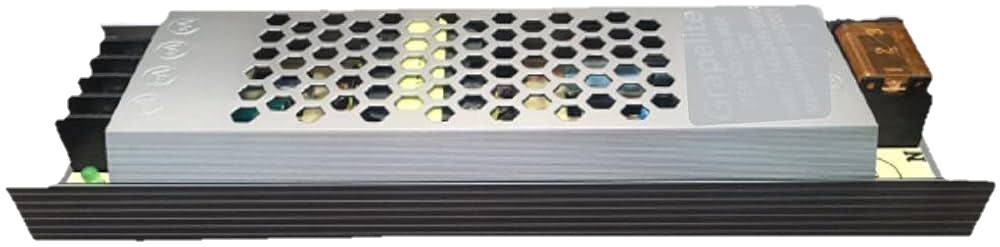
\includegraphics [
            max width = \IGXMaxWidth,
            max height = \IGXMaxHeight,
            \IGXDefaultOptionalArgs,
        ] {pics/power_supply.png}
        \captionof{figure} {
            AC to 12V DC \emph{SMPS}.
            \label{fig:powerSupply}
        }
    \end{minipage}\hfill}
\end{center}

\end{document}
